% 来源：固定候选 PDF，山东文科，PDF 第2页（印刷页323），Q20。
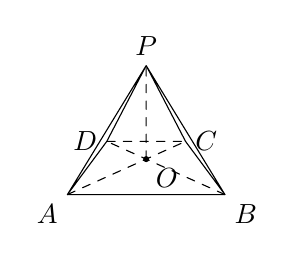
\begin{tikzpicture}[x=1cm,y=0.78cm,line cap=round,line join=round]
\coordinate (A) at (0,0); \coordinate (B) at (2,0); \coordinate (C) at (1.5,0.866); \coordinate (D) at (0.5,0.866); \coordinate (O) at (1,0.577); \coordinate (P) at (1,2.1);
\draw (A)--(B)--(C) (A)--(D) (P)--(A) (P)--(B) (P)--(C) (P)--(D);
\draw[dashed] (A)--(C) (B)--(D) (D)--(C) (O)--(P);
\fill (O) circle (1.1pt);
\node[below left] at (A) {$A$}; \node[below right] at (B) {$B$};
\node[right] at (C) {$C$}; \node[left] at (D) {$D$};
\node[above] at (P) {$P$}; \node[below right] at (O) {$O$};
\end{tikzpicture}
